\documentclass[a4paper,oneside,12pt]{article}
\usepackage{graphics,multicol}
\usepackage[latin1]{inputenc}
\usepackage[a4paper,margin=2cm,lmargin=2cm,headheight=1pt]{geometry}
\usepackage{fancyhdr}
\usepackage{amsmath,amssymb,amsfonts,amsthm, mathrsfs}
\usepackage{mathtools,bbm}
\usepackage{IEEEtrantools}
\usepackage[]{algorithm2e}
\usepackage{tikz,pgfplots,tkz-graph}
\usepackage{ifthen,calc}
\usepackage{listings,hyperref,float}
\usepackage{epsfig,epstopdf,graphicx}
\usepackage{enumerate}

\pgfplotsset{compat=newest}
\usetikzlibrary{positioning,matrix}
\interdisplaylinepenalty=2500

% Page settings
% \setlength{\oddsidemargin}{0 in}
% \setlength{\evensidemargin}{0 in}
% \setlength{\topmargin}{-0.6 in}
% \setlength{\textwidth}{6.5 in}
% \setlength{\textheight}{8.5 in}
% \setlength{\headsep}{0.75 in}
% \setlength{\parindent}{0 in}
% \setlength{\parskip}{0.1 in}

% Markov symbol X -o- Y
\newcommand{\markov}{\mathrel{\multimap}\joinrel\mathrel{-}\joinrel\mathrel{\mkern-6mu}\joinrel\mathrel{-}}
% Independent & not independent symbol X _||_ Y
\newcommand{\indep}{\mathrel{\bot}\joinrel\mathrel{\mkern-5mu}\joinrel\mathrel{\bot}}
\newcommand{\dep}{\centernot\indep}
% i.i.d.
\newcommand{\iid}{\stackrel{\mathrm{i.i.d.}}{\sim}}
% Integration d
\newcommand{\dd}{\mathop{}\!\mathrm{d}}

% Single braces
\newcommand{\agbrs}[1]{\left\langle #1 \right\rangle}	% angle braces,  	< x >
\newcommand{\rdbrs}[1]{\left( #1 \right)}				% round braces,  	( x )
\newcommand{\sqbrs}[1]{\left\lbrack #1 \right\rbrack}	% square braces, 	[ x ]
\newcommand{\clbrs}[1]{\left\lbrace #1 \right\rbrace}	% curly braces, 	{ x }

% Delimited braces
\newcommand{\agbrsv}[2]{\left\lange #1 \,\middle|\, #2 \right\rangle}	% angle braces with delimiter |,  	< x | y >, inner product
\newcommand{\rdbrsv}[2]{\left( #1 \,\middle|\, #2 \right)}				% round braces with delimiter |,  	( x | y ), conditional probability
\newcommand{\sqbrsv}[2]{\left\lbrack #1 \,\middle|\, #2 \right\rbrack}	% square braces with delimiter |,  	[ x | y ], conditional expectation
\newcommand{\clbrsv}[2]{\left\lbrace #1 \,\middle|\, #2 \right\rbrace}	% curly braces with delimiter |,  	{ x | y }, set

% Short for underline and overline
\newcommand{\udl}[1]{\underline{#1}}
\newcommand{\ovl}[1]{\overline{#1}}

% Derivative and partial derivation
\newcommand{\fracd}[2]{ \frac{\mathrm{d} #1}{\mathrm{d} #2} }
\newcommand{\fracp}[2]{ \frac{\partial #1}{\partial #2} }

% Absolute value, norm, ceil, floor, and evaluation
\newcommand{\abs}[1]{\left| #1 \right|}		% Absolute value, 	| x |
\newcommand{\norm}[1]{\left\| #1 \right\|}	% Norm, 			|| x ||
\DeclarePairedDelimiter\ceil{\lceil}{\rceil}
\DeclarePairedDelimiter\floor{\lfloor}{\rfloor}
\newcommand{\eval}[1]{\left. #1 \right|}	% Evaluation, 		f(x) |_{x=x0}

% Definition equal sign
\newcommand{\defeq}{\vcentcolon=}   % :=
\newcommand{\eqdef}{=\vcentcolon}   % =:
\newcommand{\texteq}[1]{\stackrel{#1}{=\joinrel=\joinrel=}}   % use for change of variable

% Inverse hyperbolic functions
\DeclareMathOperator\arcsinh{arcsinh}
\DeclareMathOperator\arccosh{arccosh}
\DeclareMathOperator\arctanh{arctanh}
\DeclareMathOperator\atanh{atanh}
\DeclareMathOperator\sech{sech}

% argmax and argmin
\newcommand\limit[1]{\underset{#1}{\lim}\,}
\newcommand\argmax[1]{\mathrm{arg}\,\underset{#1}{\max}\,}
\newcommand\argmin[1]{\mathrm{arg}\,\underset{#1}{\min}\,}

% Matrices
\newcommand*\pmtx[1]{\begin{pmatrix}#1\end{pmatrix}}			% Matrix with round braces
\newcommand*\bmtx[1]{\begin{bmatrix}#1\end{bmatrix}}			% Matrix with square braces
\newcommand*\vmtx[1]{\begin{vmatrix}#1\end{vmatrix}}			% Determinant of matrix
\newcommand*\spmtx[1]{\rdbrs{\begin{smallmatrix}#1\end{smallmatrix}}}	% Small matrix with round braces
\newcommand*\sbmtx[1]{\sqbrs{\begin{smallmatrix}#1\end{smallmatrix}}}	% Small matrix with square braces
\newcommand*\svmtx[1]{\abs{\begin{smallmatrix}#1\end{smallmatrix}}}		% Determinant of small matrix
\newcommand{\sizecorr}[1]{\makebox[0cm]{\phantom{$\displaystyle #1$}}}	% Get size of an expression

% Theorem environments
\newtheorem{theorem}{Theorem}
\newtheorem{corollary}[theorem]{Corollary}
\newtheorem{lemma}[theorem]{Lemma}
\newtheorem{observation}[theorem]{Observation}
\newtheorem{proposition}[theorem]{Proposition}
\newtheorem{definition}[theorem]{Definition}
\newtheorem{claim}[theorem]{Claim}
\newtheorem{fact}[theorem]{Fact}
\newtheorem{assumption}[theorem]{Assumption}

\newtheorem*{theorem*}{Theorem}
\newtheorem*{corollary*}{Corollary}
\newtheorem*{lemma*}{Lemma}
\newtheorem*{proposition*}{Proposition}
\newtheorem*{definition*}{Definition}
\newtheorem*{example*}{Example}
\newtheorem*{remark*}{Remark}
\newtheorem*{problem*}{Problem}

% Solution environment
\newenvironment{solution}{\begin{proof}[Solution]}{\end{proof}}

% Short for boldsymbol
\newcommand{\bs}[1]{\boldsymbol{#1}}

% Other frequent used operators
\def\Var{\mathsf{Var}}
\def\Cov{\mathsf{Cov}}
\def\coeff{\mathsf{coeff}}
\def\Tr{\mathsf{Tr}}
\def\rank{\mathsf{rank}}
\def\diag{\mathsf{diag}}
\def\mse{\mathsf{mse}}
\def\mmse{\mathsf{mmse}}

\def\ee{\mathbbm{e}}
\def\ii{\mathbbm{i}}
\def\EE{\mathsf{E}}
\def\FF{\mathsf{F}}
\def\SS{\mathsf{S}}
\def\UU{\mathsf{U}}
\def\xx{\mathsf{x}}
\def\pprime{{\prime\prime}}

\newcommand{\KL}[2]{D\left( #1 \,\middle|\middle|\, #2 \right)}%                   ( | )

\makeatletter
\newcommand\ztag[1]{%
\def\@currentlabel{#1}%
\gdef\tmp{%
\addtocounter{equation}{-1}%
\def\theequation{#1}}%
\aftergroup\aftergroup\aftergroup\aftergroup\aftergroup\aftergroup
\aftergroup\aftergroup\aftergroup\aftergroup\aftergroup\aftergroup
\aftergroup\aftergroup\aftergroup\aftergroup\aftergroup\aftergroup
\aftergroup\aftergroup\aftergroup\aftergroup\aftergroup\aftergroup
\aftergroup\aftergroup\aftergroup\aftergroup\aftergroup\aftergroup
\aftergroup
\tmp\IEEEyesnumber}


\pagestyle{empty}
\begin{document}
\noindent

\begin{tabular}{lcr}
  Duke University & & Math 690-40 \\  
  Homework five & \hspace{6.3cm} & F. Krzakala and L. Zdeborov\'a\\ \hline
\end{tabular}

\begin{center}
  {\Large {\bf Planted Coloring and Clustering of solutions}}
\end{center}

%\subsection*{Representing problems by graphical models}

\subsection*{Belief propagation for planted graph coloring}

In HW3 you implemented and tested BP for random graph coloring. 
In this homework the same code will come handy as you can modify it in order to verify the properties of planted coloring we defined and discussed in class. 

In particular, consider $ N $ nodes, each randomly colored with one of the the $ q $ colors. 
Call this color assignment the planted configuration $ \clbrs{ s_i^* }_{i=1}^N $. 
Create a graph $ G $ on those nodes with $ M $ edges in such a way that edges only connect different planted colors. 
Run the following tests:

\begin{enumerate}[(a)]
\item
        Initialize BP close to the uniform fixed point, i.e. $ 1/q + \epsilon^{j\to i}_s $ and iterate the equations until convergence. 
        Define converge as the time when the $ \sum_{s,(ij)} \abs{ \chi_s^{i\to j}(t+1) - \chi_s^{i\to j}(t) }/ (2qM) < \tilde \epsilon $ with suitably chosen small $\epsilon$. 
        Define overlap as
        \begin{equation}
            Q = \max_\pi \sqbrs{ \frac{1}{N} \sum_{j=1}^N \chi_{\pi(s_j^*)}^j - \frac{1}{q} } \Bigg/ \rdbrs{ 1 - \frac{1}{q} }
        \end{equation}
        Plot the overlap for $ q = 3 $ and $ q = 5 $ as a function of the average degree $ c = 2M/N $. 
        Try several sizes of graphs. 
        Describe the threshold $ c_{\mathrm{alg}}$ you observe.
\item
        Initialize BP in the planted configuration, i.e. $ \chi_s^{j\to i} = \delta_{s,s_j^*} $ and iterate the BP equations until convergence. 
        Repeat the task from the previous point and discuss the results. 
        Describe the threshold $ c_d $ you observe.
\item
        In the region where the two above initializations do not lead to the same fixed point, compare the Bethe free entropies of the two fixed points and compute and discuss the threshold $ c_{\mathrm{IT}} $.
\item
        Monitor presence of frozen variables in the BP fixed points. 
        At what average degree do frozen variables appear and how many of them? 
        Find and discuss this threshold $ c_{\mathrm{r}} $.
\end{enumerate}
\begin{solution} $\,$ 
\begin{enumerate}[(a)]
\item 
\item 
\item 
\item 
\end{enumerate}
\end{solution}



\subsection*{Large $ q $ expansion}

\begin{enumerate}[(a)]
\item 
        In class we defined the annealed (1st moment) upper bound on the colorability threshold, $ c_{\mathrm{1st}} $.
        Write the large $q$ expansion of the corresponding expression. 
\item 
        In class we also discussed that when the number of colors is large the rigidity threshold $ c_{\mathrm{r}} $ at which frozen variables appear in equilibrium scales like $ q \log(q) $.
        Persuade yourself of this fact for the random regular graphs for which we derived that the fraction of frozen variables is given as 
        \begin{equation*}
            \eta_\ell = 1 + \sum_{r=1}^{q-1} \rdbrs{ -1 }^r \binom{q-1}{r} \rdbrs{ 1 - \frac{ r \eta_{\ell+1} }{q-1} }^{d-1}
        \end{equation*}
        We remind the the rigidity threshold $ c_{\mathrm{r}} $ was defined as the largest average degree for which the above update initialized at $ \eta_\infty = 1 $ converges to $ \eta = 0 $.
        Hint: When $ q $ is large, almost all the variables are frozen already close to the threshold $ c_{\mathrm{r}} $. 
\end{enumerate}
\begin{solution} $\,$ 
\begin{enumerate}[(a)]
\item 
        From previous lecture,
        \begin{equation*}
            S_{\mathrm{annealed}} = \eval{ S_{\mathrm{Bethe}} }_{ \chi \equiv \frac{1}{q} }
            = \log(q) + \frac{c}{2} \log \rdbrs{ 1 - \frac{1}{q} }
        \end{equation*}
        Since $ c_{\mathrm{1st}} $ is the specific $ c $ at where $ S_{\mathrm{annealed}} = 0 $, we have for large $ q $
        \begin{IEEEeqnarray*}{rCl}
            c_{\mathrm{1st}}
            &=& - \frac{ 2 \log(q) }{ \log \rdbrs{ 1 - \frac{1}{q} } }
            = - \frac{ 2 \log(q) }{ -\sum_{k=1}^\infty q^{-k} / k } \\
            &=& 2 \log(q) \sqbrs{ q - \frac{1}{2} - \frac{1}{12q} + \mathrm{O} \rdbrs{ q^{-2} } }
            = (2q-1) \log(q) + \mathrm{o}(1)
        \end{IEEEeqnarray*}
\item   When $ q $ is large, almost all the variables are frozen, so instead looking at the fraction of frozen variables, we look at the fraction of free variables $ \theta_\ell \triangleq 1 - \eta_\ell $ and assume the fixed point of $ \theta $ is $ \mathrm{o}(1) $.
        Then we have
        \begin{equation*}
            \theta_\ell = -\sum_{r=1}^{q-1} \rdbrs{ -1 }^r \binom{q-1}{r} \rdbrs{ 1 - \frac{ r (1-\theta_{\ell+1}) }{q-1} }^{d-1}
        \end{equation*}
        We show that $ c_{\mathrm{r}} $ scales like $ (q-1) \sqbrs{ \log(q-1) + \log(\log(q-1)) + \alpha } $.
        To the leading exponential order, we have
        \begin{IEEEeqnarray*}{rCl}
            \binom{q-1}{r} 
            &\simeq& \exp \rdbrs{ q \mathcal{H}_\ee \rdbrs{ \frac{r}{q} } } \\
            \rdbrs{ 1 - \frac{ r (1-\theta_{\ell+1}) }{q-1} }^{d-1}
            &\simeq& \exp \rdbrs{ -\sqbrs{ \log(q) + \log(\log(q)) + \alpha } r (1-\theta_{\ell+1}) }
        \end{IEEEeqnarray*}
        So each term in the summation scales like
        \begin{equation*}
            \exp \rdbrs{ q \sqbrs{ \mathcal{H}_\ee \rdbrs{ \frac{r}{q} } - \frac{r}{q} \sqbrs{ \log(q) + \log(\log(q) + \alpha) } \rdbrs{ 1 - \theta_{\ell+1} } } }
        \end{equation*}
        In the large-$ q $ limit, it is sufficient to only look at the term with $ r = 1 $, the self-consistency equation reads:
        \begin{IEEEeqnarray*}{rCl}
            \theta 
            &=& (q-1) \exp \rdbrs{ -\rdbrs{ 1 - \theta } \sqbrs{ \log(q-1) + \log(\log(q-1)) + \alpha } } \\
            &=& \frac{1}{\log(q-1)} \ee^{-\alpha} \sqbrs{ (q-1) \log(q-1) \log(\alpha) }^\theta
            \simeq \frac{1}{\log(1-q)} \ee^{-\alpha} \rdbrs{ q-1 }^\theta
        \end{IEEEeqnarray*}
        which is solved by $ \theta = \gamma(\alpha) / \log(q-1) $ where $ \gamma(\alpha) \ee^{-\gamma(\alpha)} = \ee^{-\alpha} $.
\end{enumerate}
\end{solution}



\subsection*{Condensed phase in the random sub-cubes model}

The random-subcube model is defined by its solution space $ S \subset \clbrs{ 0,1 }^N $ (not by a graphical model). 
We define $ S $ as the union of $ \floor{ 2^{(1-\alpha)N} } $ random clusters (where $ \floor{x} $ denotes the integer value of $ x $). A random cluster $ A $ being defined as:
\begin{equation} 
    A = \clbrsv{ \vec{\sigma} }{ \sigma_i \in \pi_i^A, \quad \forall\, i \in \clbrs{ 1,\ldots,N } }
\end{equation}
where $ \pi^A $ is a random mapping:
\begin{IEEEeqnarray*}{rCl}
    \pi^A \colon \clbrs{ 1, \ldots, N } &\to& \clbrs{ \clbrs{ 0 }, \clbrs{ 1 }, \clbrs{ 0,1 } } \\
    i &\mapsto& \pi_i^A
\end{IEEEeqnarray*}
such that for each variable $ i $, $ \pi_i^A = \clbrs{ 0 } $ with probability $ p/2 $, $ \clbrs{ 1 } $ with probability $ p/2 $, and $ \clbrs{ 0,1 } $ with probability $ 1 - p $. 
A cluster is thus a random subcube of $ \clbrs{ 0,1 } $. 
If $ \pi_i^A = \clbrs{ 0 } $ or $ \clbrs{ 1 } $, variable $ i $ is said ``frozen'' in $ A $; otherwise it is said ``free'' in $ A $.
One given configuration $ \vec{\sigma} $ might belong to zero, one or several clusters. 
A ``solution'' belongs to at least one cluster. 

We will analyze the properties of this model in the limit $ N \to \infty $, the two parameters $ \alpha $ and $ p $ being fixed and independent of $ N $. 
The internal entropy $ s $ of a cluster $ A $ is defined as $ \frac{1}{N} \log_2 \rdbrs{ \abs{A} } $, i.e. the fraction of free variables in $ A $. 
We also define complexity $ \Sigma(s) $ as the (base 2) logarithm of the number of clusters of internal entropy $ s $ per variable (i.e. divide by $ N $).

\begin{enumerate}[(a)]
\item   What is the analog of the satisfiability threshold $ \alpha_s $ in this model?
\item   Compute the $ \alpha_{\mathrm{d}} $ threshold below which most configurations belong to at least one cluster.
\item   For $ \alpha > \alpha_{\mathrm{d}} $ write the expression for the complexity $ \Sigma(s) $ as a function of the parameters $ p $ and $ \alpha $. 
        Compute the total entropy defined as $ s_{\mathrm{tot}} = \max_s \sqbrsv{ \Sigma(s) + s }{ \Sigma(s) \ge 0 } $. 
        Observe that there are two regimes in the interval $ \alpha \in (\alpha_{\mathrm{d}},1) $, discuss their properties and write the value of the ``condensation'' threshold $ \alpha_{\mathrm{c}} $.
\end{enumerate}
\begin{solution} $\,$ 
\begin{enumerate}[(a)]
\item 
        The $ \alpha_{\mathrm{s}} $ is the threshold beyond which there is no ``solution''.
        A configuration is a ``solution'' if it belongs to at least one cluster, and the size of each cluster equals to $ 2^{\# \text{free variables}} \ge 1 $.

        Hence, a RSM has no ``solution'' if and only if there is zero cluster, i.e. $ \alpha > 1 $, which implies that the satisfiability threshold is $ \alpha_{\mathrm{s}} = 1 $.
\item 
        The probability that a given configuration belongs to a random cluster $ A $ is
        \begin{IEEEeqnarray*}{rCl}
            \mathbb{P} \rdbrs{ \clbrsv{ \sigma_i \in \pi_i^A }{ i \in \clbrs{ 1, \ldots, N } } }
            &=& \prod_{i=1}^N \mathbb{P} \rdbrs{ \sigma_i \in \pi_i^A } 
            = \prod_{i=1}^N \mathbb{P} \rdbrs{ \pi_i^A \in \clbrs{ \clbrs{ \sigma_i }, \clbrs{ 0,1 } } }
            = \rdbrs{ 1 - \frac{p}{2} }^N
        \end{IEEEeqnarray*}
        Therefore, the for a given configuration, the average number it belongs to is
        \begin{equation*}
            2^{(1-\alpha)N} \rdbrs{ 1 - \frac{p}{2} }^N
            = 2^{ N \sqbrs{ (1-\alpha) + \log_2 \rdbrs{ 1 - \frac{p}{2} }  } }
            = 2^{ N \sqbrs{ \log_2(2-p) - \alpha } }
        \end{equation*}
        This means in the large-$ N $ limit, if $ \alpha > \log_2(2-p) $, w.h.p. a given configuration does not belong to any random subcube, implying the clustering threshold $ \alpha_{\mathrm{d}} = \log_2(2-p) $.

        Note when $ \alpha < \alpha_{\mathrm{d}} $, almost every configuration belongs to at least one cluster, so almost all configurations are ``solutions'', $ s_{\mathrm{tot}} = \frac{1}{N} \log_2 \rdbrs{ \abs{S} } = 1 $.
\item 
        The probability that a cluster has internal entropy $ s $ is
        \begin{equation*}
            \mathcal{P}(s) = \binom{N}{sN} \rdbrs{ 1 - p }^{sN} p^{(1-s)N}
        \end{equation*}
        Let $ \mathcal{N}(s) $ be the number of clusters with internal entropy $ s $, then it is easy to see $ \mathcal{N}(s) \sim \mathsf{Binomial} \rdbrs{ 2^{(1-\alpha)N}, \mathcal{P}(s) } $, i.e.
        \begin{IEEEeqnarray*}{rCl}
            \mathbb{E} \sqbrs{ \mathcal{N}(s) }
            &=& 2^{(1-\alpha)N} \mathcal{P}(s), \qquad
            \Var \rdbrs{ \mathcal{N}(s) }
            = 2^{(1-\alpha)N} \mathcal{P}(s) \rdbrs{ 1 - \mathcal{P}(s) }
        \end{IEEEeqnarray*}
        By Markov and Chebyshev's inequality, we have
        \begin{IEEEeqnarray*}{rCl}
            \mathbb{P} \rdbrs{ \mathcal{N}(s) \ge 1 } 
            &\le& \mathbb{E} \sqbrs{ \mathcal{N}(s) } \\
            \mathbb{P} \rdbrs{ \abs{ \frac{\mathcal{N}(s)}{ \mathbb{E}\sqbrs{ \mathcal{N}(s) } } - 1 } > \varepsilon }
            &\le& \frac{ \Var \rdbrs{ \mathcal{N}(s) } }{ \clbrs{ \mathbb{E}\sqbrs{ \mathcal{N}(s) } }^2 \varepsilon^2 }
            \le \frac{1}{ 2^{ N (1-\alpha) } } \varepsilon^2 \mathcal{P}(s), \quad \forall\, \varepsilon > 0
        \end{IEEEeqnarray*}
        These equation prove the the random quantity $ \frac{1}{N} \log \rdbrs{ \mathcal{N}(s) } $ concentrates around its expectation in the large-$ N $ limit, that is,
        \begin{equation*}
            \limit{N \to \infty} \frac{1}{N} \log \rdbrs{ \mathcal{N}(s) } =
            \begin{cases}
                \Sigma(s) \defeq 1 - \alpha - \KL{s}{1-p} , &\text{ if } \Sigma(s) \ge 0 \\
                -\infty, &\text{ otherwise }
            \end{cases}
        \end{equation*}
        where the binary KL divergence is defined as
        \begin{equation*}
            \KL{x}{y} = x \log_2 \rdbrs{ \frac{x}{y} } + (1-x) \log_2 \rdbrs{ \frac{1-x}{1-y} }
        \end{equation*}
        Now we consider the regime $ \alpha > \alpha_{\mathrm{d}} $,
        The total entropy is given by a saddle-point estimation, to the leading exponential order we have
        \begin{IEEEeqnarray*}{rCl}
            \sum_A 2^{N s(A)}
            &\simeq& N \int_s \dd s ~ 2^{ N \sqbrs{ \Sigma(s) + s } } \mathbb{I} \rdbrs{ \Sigma(s) \ge 0 }
        \end{IEEEeqnarray*}
        Although it seems to over count the solutions since a configuration may belong to several clusters and this sum just adds the cluster size, but in the regime $ \alpha > \alpha_{\mathrm{d}} $ it is valid because since in every cluster the fraction of solutions belonging to more than one cluster is exponentially small.

        Taking derivative of $ \Sigma(s) + s $ and setting it to zero solves
        \begin{equation*}
            \fracp{}{s} \sqbrs{ \Sigma(s) + s } = \log_2 \rdbrs{ \frac{1-p}{p} \frac{1-s}{s} } + 1
            \quad \Rightarrow \quad
            \tilde{s} = \frac{2(1-p)}{2-p}, \quad 
            \Sigma(\tilde{s}) = \frac{p}{2-p} - \alpha + \log_2(2-p)
        \end{equation*}
        \begin{itemize}
        \item   When $ \Sigma(\tilde{s}) > 0 $, i.e. $ \alpha < \alpha_{\mathrm{c}} \defeq \frac{p}{2-p} + \log_2(2-p) $, the correct maximizer is $ s^* = \tilde{s} $
                \begin{equation*}
                    s_{\mathrm{tot}} = \Sigma(\tilde{s}) + \tilde{s} = 1 - \alpha + \log_2(2-p)
                \end{equation*}
        \item   When $ \Sigma(\tilde{s}) < 0 $, the correct maximizer $ s^* = s_M = \max \clbrsv{ s }{ \Sigma(s) >= 0 } $, which is the cross point of $ \Sigma(s) $ and the $ x $-axis
                \begin{equation*}
                    s_{\mathrm{tot}} = \Sigma(s_M) + s_M = 0 + s_M = s_M
                \end{equation*}
        \end{itemize}

        Therefore, there are four different phases
        \begin{enumerate}[(1)]
        \item   
                Liquid phase: $ \alpha < \alpha_{\mathrm{d}} $, almost all configurations are solutions, this can be also seen from $ s_{\mathrm{tot}} = 1 $
        \item   
                Clustered phase: $ \alpha_{\mathrm{d}} < \alpha < \alpha_{\mathrm{c}} $, the solutions set $ S $ is partitioned into exponentially many non-overlapping clusters.
                Most solutions are in the $ \ee^{N \Sigma(\tilde{s})} $ clusters with internal entropy $ \tilde{s} $.
        \item   
                Condensed clustered phase: $ \alpha_{\mathrm{c}} < \alpha < \alpha_{\mathrm{s}} $, the solutions set $ S $ is partitioned into exponentially many non-overlapping clusters.
                However, most solutions are in the clusters with internal entropy $ s_M $.
                The number of such clusters is not exponentially large, as $ \Sigma(s_M) = 0 $.
        \item   
                Unsatisfiable phase: $ \alpha > \alpha_{\mathrm{s}} $, there is no cluster, and thus no solutions.
        \end{enumerate}
        \begin{figure}[H]
            \centering
            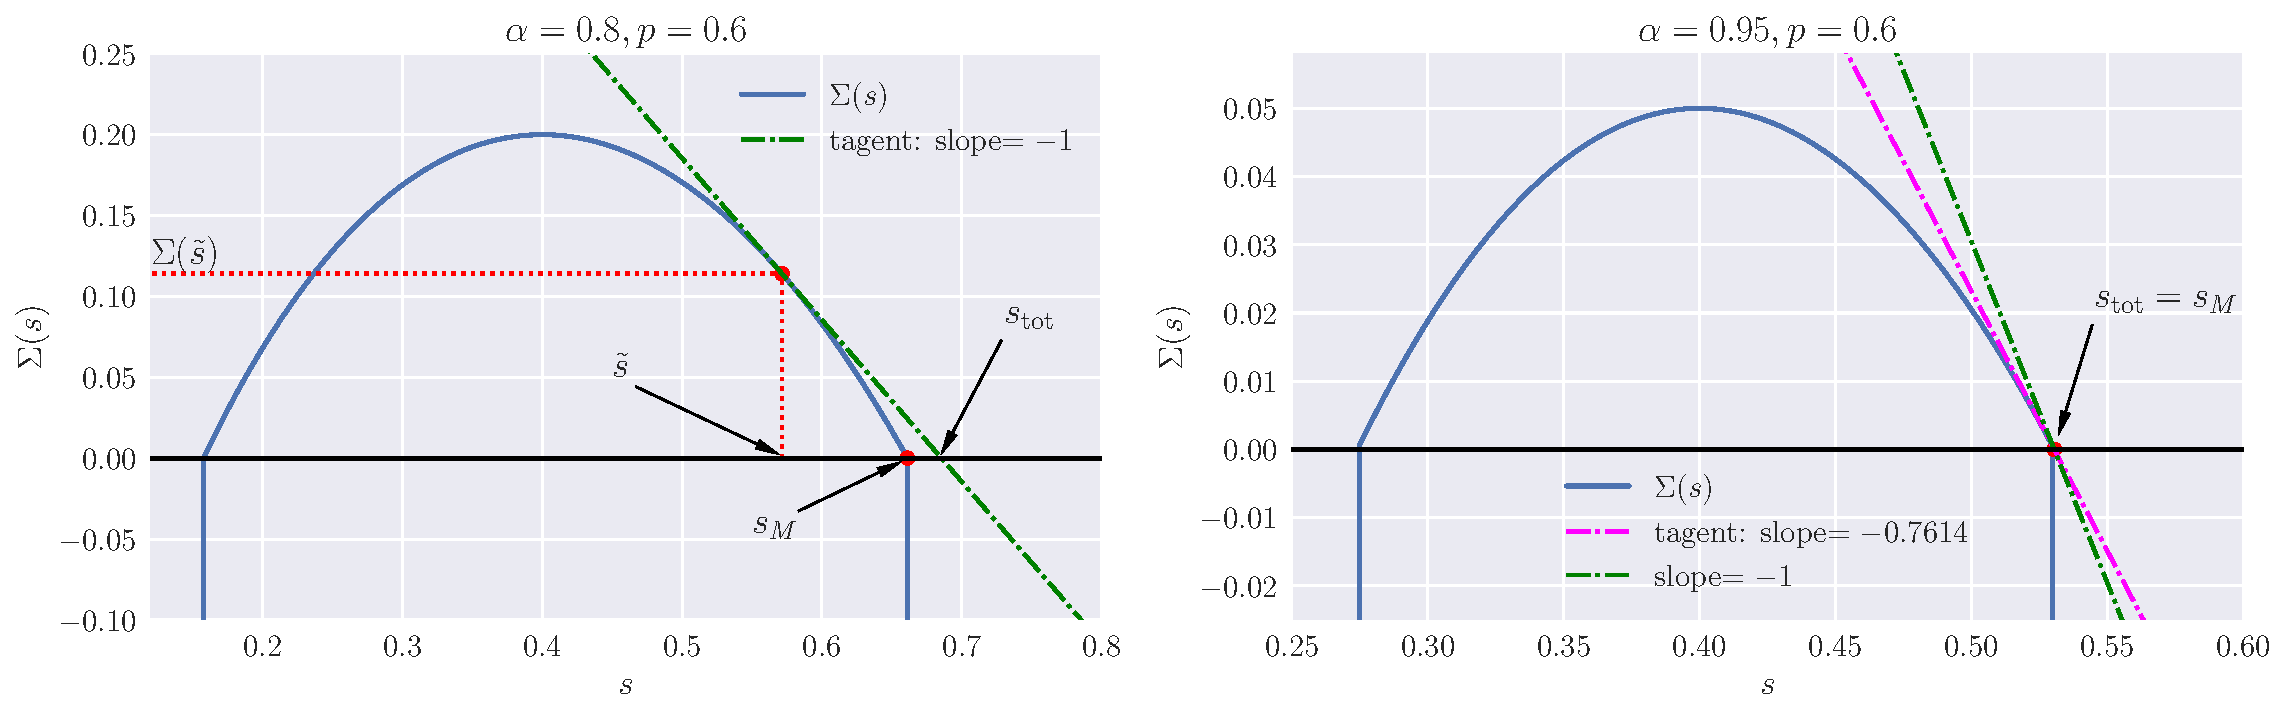
\includegraphics[width=\textwidth]{hw5/hw5_3(c)1.pdf}
            \vspace{-10mm}
            \caption{Complexity function $ \Sigma(s) $ under clustered phase (left, $ \alpha = 0.8, p = 0.6 $) and condensed clustered phase (right, $ \alpha = 0.95, p = 0.6 $)}
        \end{figure}
        \begin{figure}[H]
            \centering
            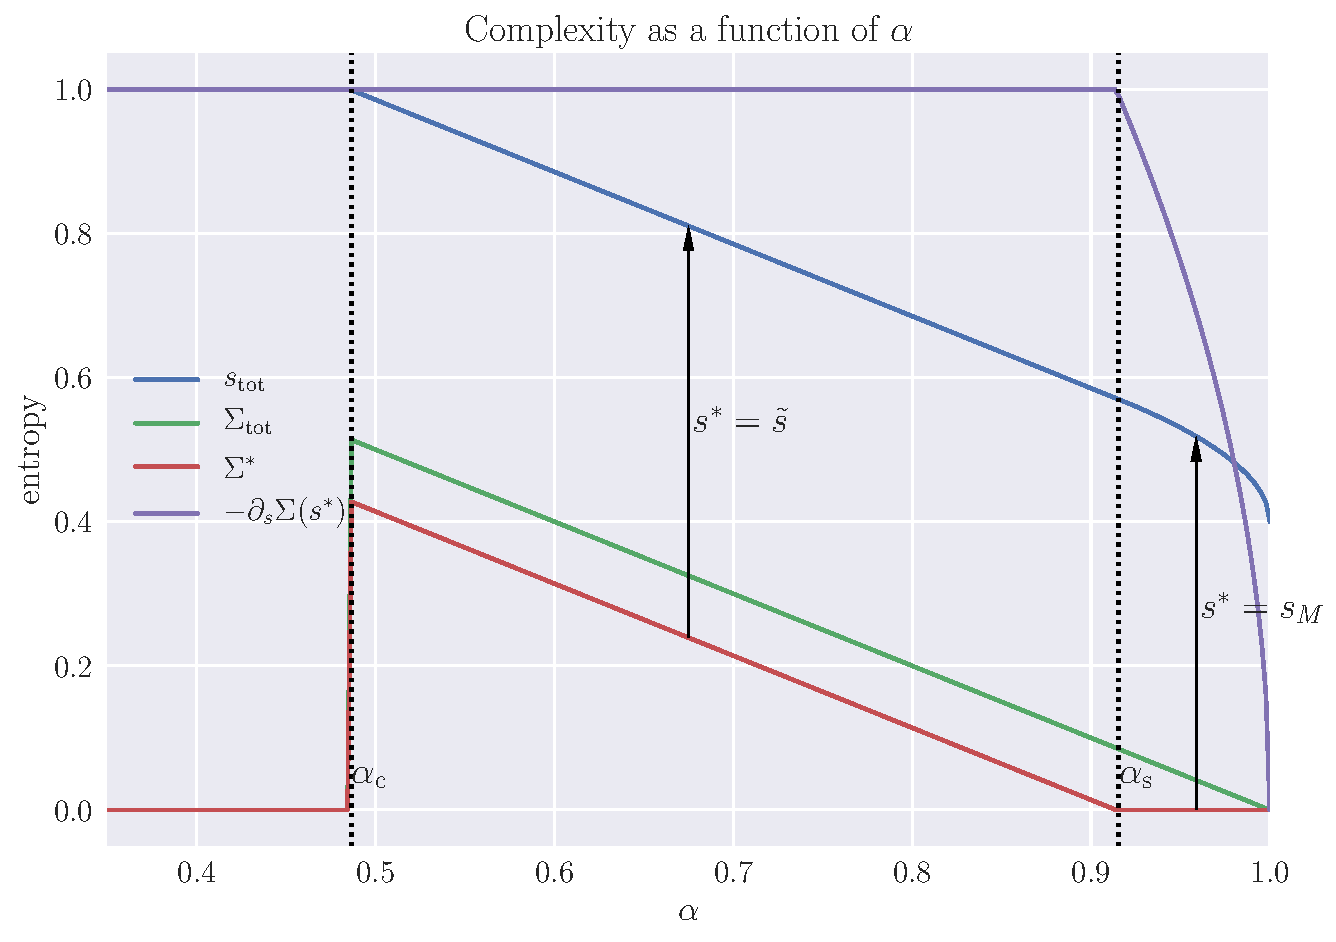
\includegraphics[width=0.6\textwidth]{hw5/hw5_3(c)2.pdf}
            \caption{Complexity as a function of $ \alpha $ for $ p = 0.6 $.}
        \end{figure}
\end{enumerate}
\end{solution}


\end{document}